\section{Results and Discussion}
\label{sec:results_and_discussion}
\hspace{8pt}
To prove that the filtering stage of the system is working properly, an AC sweep was done from 0 Hz to 10 GHz. For this analysis, real-life values of resistors and capacitors were used. From Fig~\ref{fig:fdt_design_circuit}, the value of the resistor R1\_S1 was changed from $20.5~k\Omega$ to $20 k\Omega$ and the capacitor C1\_S1 from 1.4 nF to 1.5 nF. In Fig~\ref{fig:filter_multisim} the simulated circuit in NI Multisim is shown.

\begin{figure}[H]
    \centering
    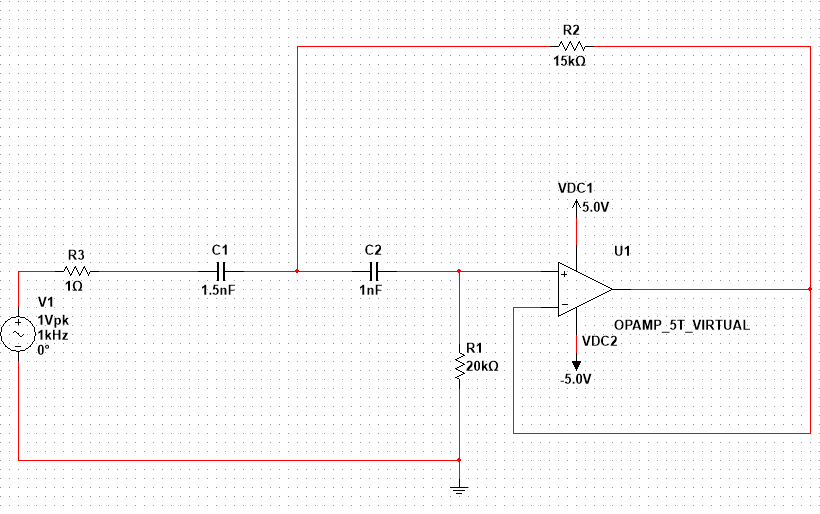
\includegraphics[width=0.8\linewidth]{filter_multisim}
    \caption{Filtering stage circuit simulated in NI Multisim}
~\label{fig:filter_multisim}
\end{figure}

The OPA2186 operational amplifier doesn't exist in NI Multisim libraries, so a virtual operational amplifier is required. The parameters of the OPA2186 were taken from the vendor datasheet and set as in Fig~\ref{fig:opa2186_parameters}.

\begin{figure}[H]
    \centering
    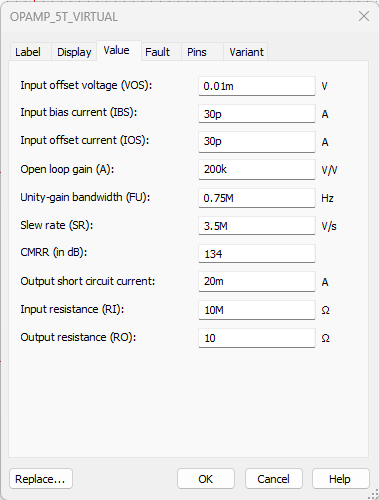
\includegraphics[width=0.48\linewidth]{opa2186_parameters}
    \caption{OPA2186 parameter configuration for the virtual operational amplifier of NI Multisim}
~\label{fig:opa2186_parameters}
\end{figure}

After running the AC sweep analysis over the filtering stage of the system, the Bode plot of Fig~\ref{fig:ac_sweep_analysis} is obtained. The gain and phase shift of the filter as a function of the frequency is similar to the expected results shown in Fig~\ref{fig:fdt_design:magnitude} and ~\ref{fig:fdt_design:phase}. The Bessel response provides a maximally flat passband with minimal overshooting and ringing, without exhibiting resonant peaks. Also, the phase shift is nearly linear with frequency, representing a minimal distortion.

\begin{figure}[H]
    \centering
    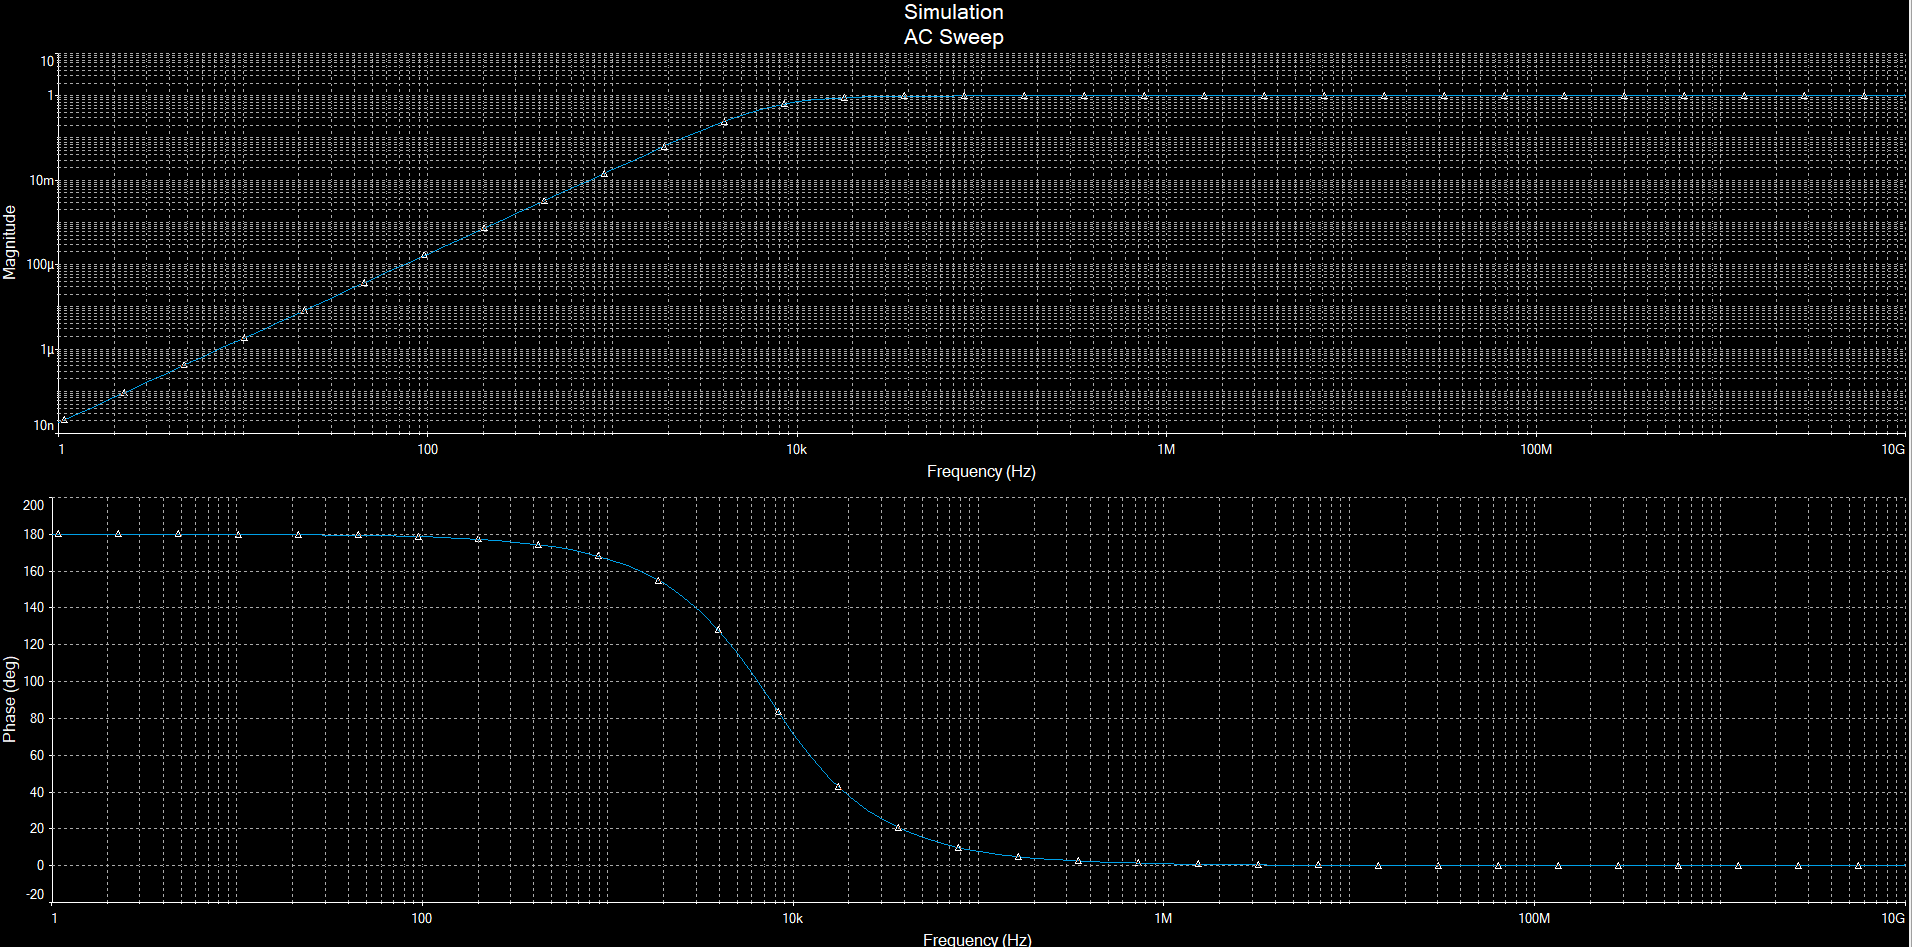
\includegraphics[width=1\linewidth]{ac_sweep_analysis}
    \caption{AC sweep analysis of the filtering stage of the system in NI Multisim}
~\label{fig:ac_sweep_analysis}
\end{figure}

The circuit for the amplification stage is shown in Fig~\ref{fig:amp_multisim}. Parameters for the virtual operational amplifier are obtained from the LM358 datasheet and are shown in Fig~\ref{fig:lm358_parameters}.

\begin{figure}[H]
    \centering
    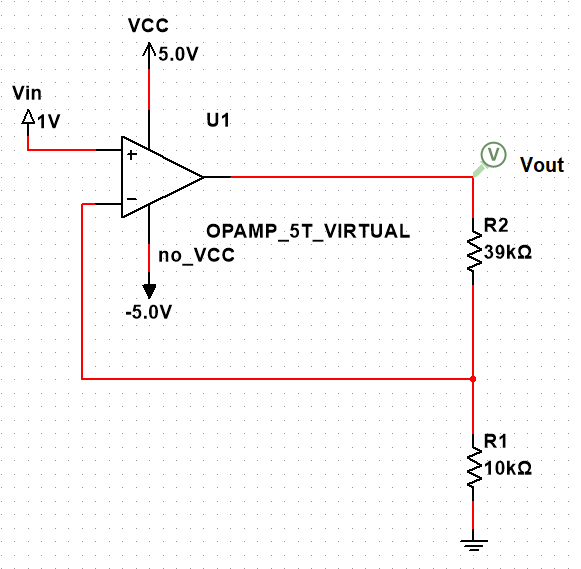
\includegraphics[width=0.5\linewidth]{amp_multisim}
    \caption{Amplification stage circuit simulated in NI Multisim}
~\label{fig:amp_multisim}
\end{figure}

\begin{figure}[H]
    \centering
    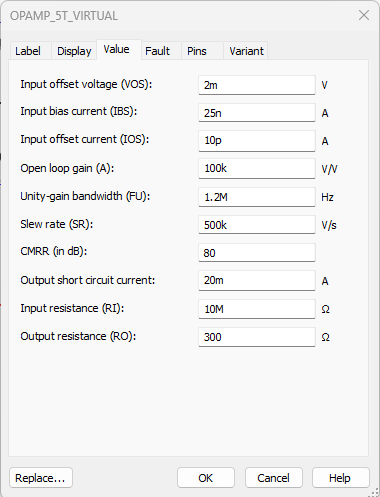
\includegraphics[width=0.48\linewidth]{lm358_parameters}
    \caption{LM358 parameter configuration for the virtual operational amplifier of NI Multisim}
~\label{fig:lm358_parameters}
\end{figure}

After running a DC sweep analysis, changing the input voltage from 0V to 1V in steps of 1mV, the plot of Fig~\ref{fig:dc_sweep_amplification} is obtained. In this plot, the expected behavior for the operational amplifier is observed. The amplification stage has an output voltage near 0 V when the input voltage is 0 V, and an output voltage near 4.9 V when the input voltage is 1 V. There is still an output offset voltage of -8.84 mV when the input voltage is 0 V, but this can be compensated adding a current source with a value of 226.56 nA.

\begin{figure}[H]
    \centering
    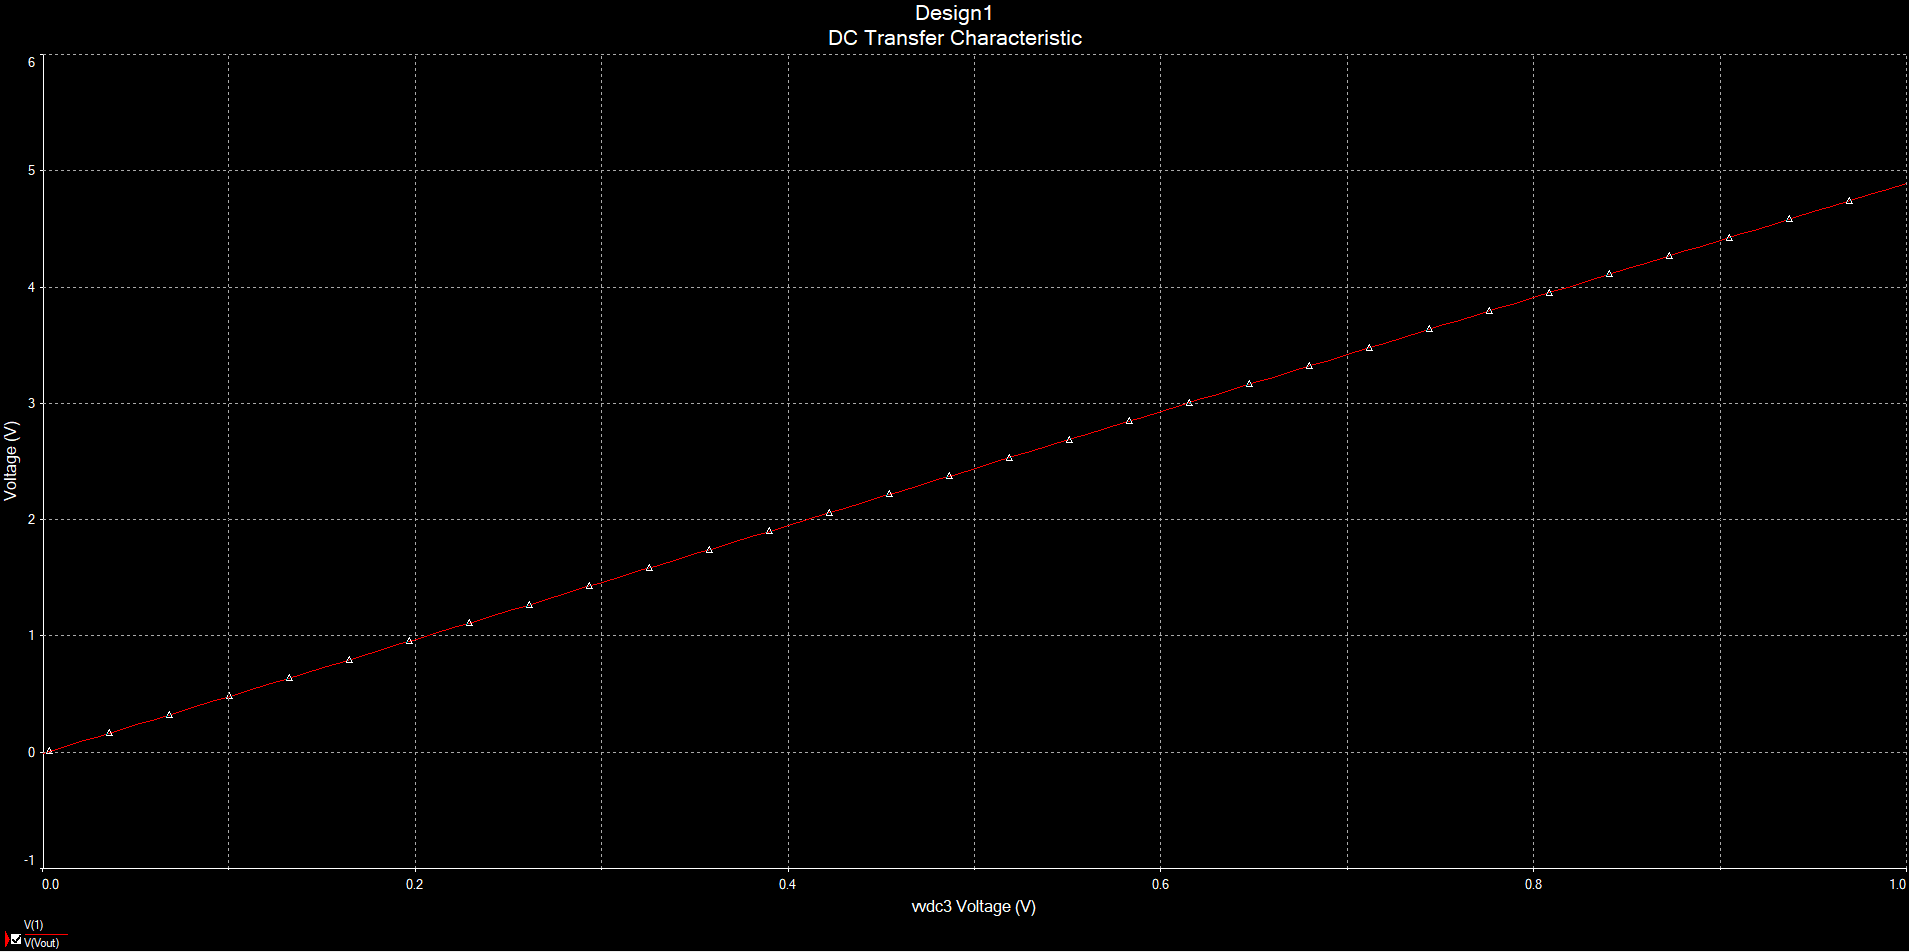
\includegraphics[width=1\linewidth]{dc_sweep_amplification}
    \caption{DC sweep analysis of the amplification stage of the system in NI Multisim}
~\label{fig:dc_sweep_amplification}
\end{figure}


\begin{figure}[H]
    \centering
    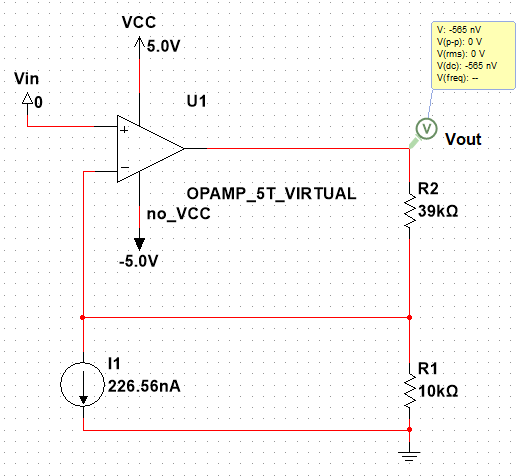
\includegraphics[width=0.5\linewidth]{amp_comp_multisim}
    \caption{DC sweep analysis of the amplification stage of the system in NI Multisim}
~\label{fig:amp_comp_multisim}
\end{figure}



